% !TEX root = ../thesis.tex

\chapter{Vorhandene Arbeit}
\label{ch:vorhandene-arbeit}

In diesem Kapitel werden die Kernaufgaben dieser Arbeit behandelt:
Registrierung von mehreren Punktwolken in einem Koordinatensystem (\ref{sec:registration}), Segmentierung in einzelne Cluster (\ref{sec:segmentation}) und Triangulation der Wolke zu einem Polygonnetz (\ref{sec:triangulation}).

Neben Erläuterung der Problematik wird ein Blick auf die aktuelle Forschung zum jeweiligen Thema geworfen.
Außerdem werden mögliche Lösungsansätze auf ihren praktischen Nutzen untersucht und die Vor- und Nachteile diskutiert.


\section{Registrierung von Punktwolken}
\label{sec:registration}

Beim Erfassen von Objekten in der Realität, beispielsweise mithilfe eines Laserscanners, werden häufig Punktwolken aus verschiedenen Perspektiven aufgenommen.
Der Grund dafür ist, dass aus einer Scanposition nicht immer die gesamte Oberfläche sichtbar ist, etwa aufgrund von Verschattungen durch das Objekt selbst.
Weiterhin können so Reflektionen und spiegelnde Oberflächen wie auch Hintergrundrauschen gemittelt werden, sodass weitgehend robuste Daten erhalten werden.

In vielen Fällen ist die zugehörige Aufnahmeposition nicht bekannt, unzureichend genau oder es liegt kein kalibriertes System vor.
Aus diesem Grund müssen die erfassten Punktwolken erst in ein globales Koordinatensystem gebracht werden.
Diesen Prozess nennt man Registrierung.


\subsection{Lokale Registrierung}
\label{subsec:local-registration}

Bei der lokalen Registrierung von zwei Punktwolken müssen diese bereits grob aneinander ausgerichtet sein.
Der Registrierungsalgorithmus verfeinert diese Ausrichtung dann weiter und findet ein lokales Minimum.
Einer der bekanntesten Algorithmen zur lokalen Registrierung ist \ac{ICP} und seine vielen verschiedenen Varianten.


\subsubsection{\acl{ICP}}
\label{subsubsec:icp}

\ac{ICP} \cite{besl1992method} ist der wohl bekannteste Algorithmus zur lokalen Registrierung von Punktwolken.
Im Laufe der Zeit wurden zahlreiche Varianten und Optimierungen dafür entwickelt, die beispielsweise auch die Normalen in den Punkten in Betracht ziehen oder besonders resistent gegen statistische Ausreißer sind \cite{rusinkiewicz2001efficient, bouaziz2013sparse, munch2010modified}. Unter anderem existiert auch eine vorhandene Implementierung in der \ac{PCL} \cite{holz2015registration}.

\autoref{alg:icp} beschreibt, wie Punktwolke $A$ an Punktwolke $B$ registriert werden kann.
Der Ablauf lässt sich folgendermaßen grob erklären:

\begin{enumerate}
\item $A$ wird iterativ durch Anwendung von Translationen und Rotationen in eine neue Position gebracht, zum Beispiel mithilfe von Quaternionen \cite{horn1987closed}.
\item Zu jedem Punkt $p \in A$ wird der Punkt $q \in B$ gesucht, der den geringsten Abstand $e = \|p - q\|$ von $p$ hat.
\item Berechne den Fehler $\varepsilon = \sum e^2$, Standard ist die Summe der Residuenquadrate.
\item Wiederholung, bis eine der Abbruchbedingungen eintritt.
\end{enumerate}

Die Abbruchbedingungen sind dabei je nach Implementierung unterschiedlich.
Meist terminiert der Algorithmus jedoch, wenn

\begin{itemize}
\item $\varepsilon < \alpha$ mit Grenzwert $\alpha > 0$ für den Restfehler
\item $\Delta e > \delta$, mit $\delta > 0$ als Grenzwert für die Änderung des Fehlers
\item eine festgelegte Zahl von Iterationen abgelaufen ist.
\end{itemize}

Selbstverständlich lassen sich beliebig viele zusätzliche Kriterien definieren, beispielsweise eine festgelegte maximale Laufzeit.


\begin{algorithm}[ht]
\caption{\acl{ICP}}
\label{alg:icp}
\begin{algorithmic}
\Function{ICP}{$cloud1, cloud2$}
	\State $PointMap \gets \emptyset$
	\ForAll{$p \in cloud1$}
	\Comment{Find corresponding points}
		\State $q \gets$ \Call{findNearestNeighbor}{$cloud2, p$}
		\If{\Call{dist}{$p, q$} $< maxDist$}
			\State \Call{$PointMap$.add}{$p, q$}
		\EndIf
	\EndFor
	\While{termination Criteria not met}
	\Comment{Now, align the clouds}
		\State $t \gets$ \Call{estimateTransformation()}{}
		\State \Call{$cloud1$.transform}{$t$}
		\State $\varepsilon \gets$ \Call{calculateError}{$PointMap$}
	\EndWhile
\EndFunction
\Function{calculateError}{$PointMap$}
	\State $\varepsilon \gets 0$
	\ForAll{$p, q \in PointMap$}
		\State $e \gets \|p - q\| = \sqrt{(p_x - q_x)^2 + (p_y - q_y)^2 + (p_z - q_z)^2}$
		\State $\varepsilon \gets \varepsilon + e^2$
	\EndFor
	\State \Return{$\varepsilon$}
\EndFunction
\end{algorithmic}
\end{algorithm}


\subsubsection{Kinect Fusion}
\label{subsubsec:kinfu}

Durch die Veröffentlichung der Microsoft Kinect im Jahr 2010 wurde aufgrund ihres niedrigen Preises erstmals der breiten Masse der Zugang zu Tiefenkameras ermöglicht \cite[1:55]{kinfuTalkYoutube}.
Die Kinect ist eine 3D-Kamera, welche ursprünglich für die Nutzung im Entertainment- und Gamingbereich entwickelt worden ist.
Bestehend aus einem Lichtemitter, Infrarotsensor, einer 2D-RGB-Kamera und weiteren Sensoren, liefert sie 3D-Daten bei einer Bildwiederholfrequenz von 30 Hz.
Neben dem ursprünglichen Anwendungsgebiet findet sie heute auch in vielen anderen, auch wissenschaftlichen Bereichen Anwendung, beispielsweise bei der Aufzeichnung geomorphologischer Daten \cite{mankoff2013kinect}.

\ac{KinFu} ist das Ergebnis einer Forschungsarbeit von Microsoft Research \cite{izadi2011kinectfusion} und bietet eine Möglichkeit, mithilfe der Kinect 3D-Rekonstruktionen in Echtzeit durchzuführen.
\ac{KinFu} kombiniert dabei die lokale Registrierung durch den \ac{ICP}-Algorithmus mit einem \ac{TSDF}.
Ein \ac{TSDF} ist im Grunde genommen nichts anderes als ein Voxel Grid.
Während der Wert eines Voxel im ursprünglichen Voxel Grid Informationen über die Daten im betreffenden Voxel enthält, wird hier die Entfernung zur nächsten Oberfläche gespeichert \cite{curless1996volumetric}.
Somit stehen innerhalb des Objekts negative Werte in den Voxeln und außerhalb positive Werte.
Die Oberfläche wird damit implizit durch den Nulldurchgang der Distanzen in den Voxeln definiert.

Dies ermöglicht bei einer relativ geringen Auflösung dennoch eine recht genaue Rekonstruktion der vorhandenen Oberflächen.
Um dies zu erreichen, werden die Distanzen in den Voxeln interpoliert und Fehler durch die geringe Auflösung oder Sensorrauschen minimiert.

\begin{figure}[ht]
	\centering
	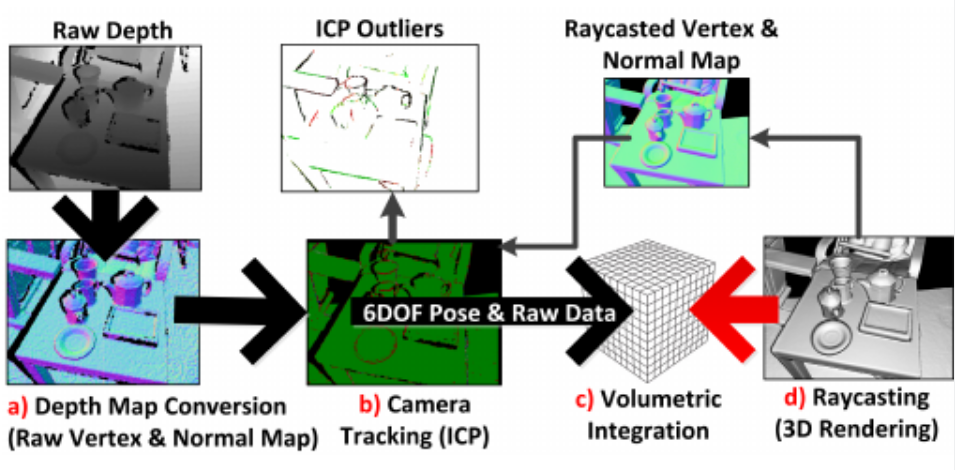
\includegraphics[width=0.66\textwidth, frame]{images/kinfu-integration.png}
	\caption{Integration eines Tiefenbilds in \ac{KinFu}. Entnommen aus \cite{izadi2011kinectfusion}}
	\label{fig:kinfu-integration}
\end{figure}

Durch eine schnelle GPU-Implementierung auf Basis von \ac{CUDA} erreicht \ac{KinFu} dabei eine Integration neuer Tiefenbilder bei 30 Hz, der Bildwiederholfrequenz der Kinect.
Somit ist die zeitliche Differenz zwischen zwei Aufnahmen sehr niedrig.
Es wird davon ausgegangen, dass die Kamera handgeführt (bzw. mit geringer Geschwindigkeit bewegt) wird, daher hält sich auch die räumliche Distanz zwischen einzelnen Frames in Grenzen.
Aufgrund dieser Gegebenheiten reicht bei \ac{KinFu} eine lokale Registrierung aus, es kann also direkt \ac{ICP} verwendet werden.

In \autoref{fig:kinfu-integration} ist der Ablauf der Integration eines neuen Tiefenbilds ins \ac{TSDF} bei \ac{KinFu} dargestellt.
Das Tiefenbild wird zunächst in eine Punktwolke konvertiert.
Diese wird anschließend durch \ac{ICP} registriert, um dann unter Bildung eines Mittelwerts in das \ac{TSDF} integriert zu werden.
Zur Darstellung der Szene wird dieses anschließend mithilfe eines Raycasters gerendert.


Es gibt zahlreiche Optimierungen und veränderte Versionen von \ac{KinFu}.
Unter anderem gibt es in der \ac{PCL} eine freie Implementierung \cite{pirovano2012kinfu}.
Eine optimierte Version ist beispielsweise Chisel \cite{klingensmith2015chisel}, wo eine effizientere Voxelstrategie verwendet wird.
Weiterhin ist Chisel eine reine CPU-Implementierung, was die Nutzung auf Mobilgeräten ohne Grafikkarte ermöglicht.

Die in dieser Arbeit verwendete Implementierung ist \ac{YAK}.
\ac{YAK} ist eine auf \ac{ROS} angepasste Version von \ac{KinFu}, um Trajectory Waypoints für die Robotersteuerung zu errechnen \cite{schornak2019yak}.
Die Verwendung von \ac{KinFu} in industriellen Robotikanlagen ist in vielerlei Hinsicht sinnvoll:
\begin{itemize}
\item Objekte können aus mehreren Perspektiven gescannt werden, was eine bessere Darstellung der Szene liefert.
\item Rauschen durch den Bildsensor wird aufgrund der Mittelwertbildung minimiert.
Das Ergebnis ist ein glatteres und realistischeres Modell.
\item Durch die GPU-Implementierung können Tiefenbilder in Echtzeit integriert werden, was insbesondere bei Robotikanwendungen ein großer Vorteil ist.
\item Ein häufig in der Bildverarbeitung auftretendes Problem sind reflektierende bzw. spiegelnde Oberflächen.
Die betroffenen Regionen können oft nur falsch, verzerrt oder gar nicht modelliert werden.
Da hier eine Aufnahme aus mehreren Perspektiven möglich ist, können derartige Fehler weitestgehend vermieden werden. In \autoref{fig:yak-reflecting-model} ist dies an einem Beispiel besonders gut sichtbar.
\end{itemize}

\begin{figure}[ht]
	\centering
	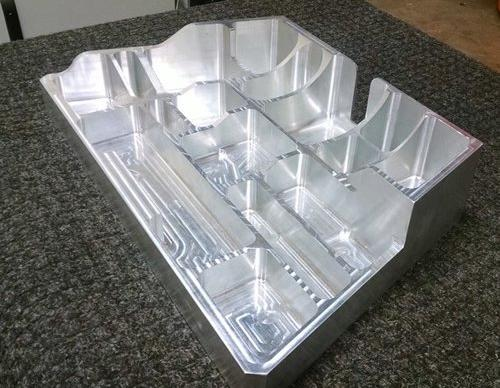
\includegraphics[width=0.4\textwidth]{images/yak-reflecting-scene.jpg}
	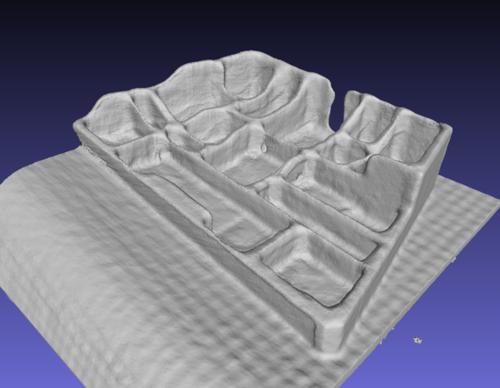
\includegraphics[width=0.4\textwidth]{images/yak-reflecting-reconstruction.png}
	\caption{Szene und Rekonstruktion eines reflektierenden Objekts durch \ac{YAK}. Entnommen aus \cite{schornak2019yak}}
	\label{fig:yak-reflecting-model}
\end{figure}

Der Vorteil der Echtzeitintegration ist jedoch gleichzeitig auch ein großes Problem.
In industriellen Robotikanlagen sind nur selten Grafikkarten verbaut.
Eine Hochleistungs-GPU-Einheit mit \ac{CUDA}-Unterstützung ist dabei aber unerlässlich, da sonst nur ein Bruchteil der Geschwindigkeit erreicht werden kann.


\subsection{Globale Registrierung}
\label{subsec:global-registration}

Bei der globalen Registrierung müssen sich die beiden Punktwolken nicht nahe der endgültigen Ausrichtung befinden - Translation und Rotation können beliebig sein.
Ein Nachteil ist jedoch, dass die globale Registrierung oft nur eine Grobregistrierung bietet, also keine optimalen Ergebnisse liefert.
Aus diesem Grund bietet es sich meist an, anschließend noch eine lokale Registrierung zur Verbesserung der Ergebnisse durchzuführen.

Zur globalen Registrierung von Punktwolken existieren verschiedene Ansätze \cite{chaudhury2015global, zhou2016fast, rusu2009fast}.
Die in dieser Arbeit verwendete Methode ist Super4PCS \cite{mellado2014super4pcs}, eine optimierte Version von \ac{4PCS} \cite{aiger2008fpcs}.
Dieser Ansatz wird verwendet, da die vorhandene Implementierung \ac{OpenGR} \cite{mellado2018opengr} über einen Wrapper bereits zur \ac{PCL} kompatibel ist.

%TODO 4PCS Funktionsweise erklären


\section{Segmentierung}
\label{sec:segmentation}

Ziel der Segmentierung ist es, zusammengehörende Bildregionen zu identifizieren und durch Zuweisung verschiedener Klassen voneinander zu trennen.
Dies ist, insbesondere in der 2D-Bildverarbeitung, ein altes Problem, für das es viele verschiedene Lösungsansätze gibt.
Auch im dreidimensionalen Raum ist eine Segmentierung häufig notwendig.
In vielen Fällen gibt es dabei nicht eine beste Methode - die Objektart, -größe, -form und viele weitere Faktoren beeinflussen die Wahl eines geeigneten Ansatzes.

Die Forschung ist in diesem Bereich weiterhin sehr aktuell:
Beispielsweise zeigen \citeauthor{uckermann2012real} einen Versuch, in Echtzeit und ohne vorher bekannte Objekte zu segmentieren \cite{uckermann2012real}.
Eine Übersicht bieten \citeauthor{nguyen20133d}, die verschiedene Varianten vergleichen und die Vor- und Nachteile diskutieren \cite{nguyen20133d}.
In den letzten Jahren findet auch verstärkt Forschung zur Segmentierung mithilfe von Neuronalen Netzen statt \cite{te2018rgcnn}.

% Segmentierung auf Meshes
%TODO
Survey \cite{shamir2008survey}, SDF \cite{shapira2008consistent}


\subsection{3D-Ansätze}
\label{subsec:3d-segmentation}

Im dreidimensionalen Raum gibt es viele verschiedene Eigenschaften (Features), die zur Segmentierung von Punktwolken herangezogen werden können.
Es spielt selbstverständlich die Distanz zwischen den Punkten eine Rolle, aber auch andere Faktoren wie Normalenorientierung, Farbe oder Krümmung bieten in vielen Fällen nützliche Zusatzinformationen.

Im Folgenden werden die zwei getesteten Methoden \ac{ECE} und Region Growing erklärt.
Eine gute Übersicht über die beiden Verfahren bietet auch \citeauthor{RusuDoctoralDissertation} in \cite[S.88--93]{RusuDoctoralDissertation}.

\subsubsection{\acl{ECE}}
\label{subsubsec:euclidean-cluster-extraction}

Diese Methode der Segmentierung im dreidimensionalen Raum ist sehr einfach.
Sie basiert auf der Annahme, dass Punkte so lange zu einem Cluster gehören, so lange ihr Abstand unter einem Grenzwert liegt.

In \autoref{alg:euclidean-cluster-extraction} beschreibt, wie die Cluster $\mathcal{C} \subseteq P$ für die Punktwolke $P$ nach \cite[S.89f]{RusuDoctoralDissertation} errechnet werden.

\begin{algorithm}
\caption{\acl{ECE}}
\label{alg:euclidean-cluster-extraction}
\begin{algorithmic}
\State $\mathcal{C} \gets \emptyset$
\Comment{list of clusters}
\State $\mathcal{Q} \gets \emptyset$
\Comment{current cluster queue}
\ForAll{$p \in P$}
	\State $\mathcal{Q} \gets p$
	\ForAll{unprocessed points $q \in \mathcal{Q}$}
		\State mark $q$ as processed
		\State $\mathcal{N} \gets$ \Call{nearestKSearch}{$q, \delta$}
		\Comment{$\delta$-region around q}
		\State $\mathcal{Q} \gets$ all unprocessed points in $\mathcal{N}$
	\EndFor
	\State $\mathcal{C} \gets \mathcal{Q}$
	\Comment{add processed queue to clusters}
	\State $\mathcal{Q} \gets \emptyset$
	\Comment{reset the queue}
\EndFor
\State \Return{$\mathcal{C}$}
\end{algorithmic}
\end{algorithm}

\subsubsection{Region Growing}
\label{subsubsec:region-growing}


\subsection{Watershed-Algorithmus}
\label{subsec:watershed}


\section{Triangulierung}
\label{sec:triangulation}

Die Konvertierung einer Datenstruktur zu einem aus Polygonen bestehenden Mesh nennt sich Triangulierung.
Gerade bei der Triangulierung von Punktwolken gibt es jedoch nicht immer eine einzelne korrekte Lösung dieses Problems.
Es ist beispielweise nicht immer sichergestellt, dass jeder Punkt auch tatsächlich die zu rekonstruierende Oberfläche darstellt - Rauschen, Reflektionen oder sonstige Fehler können auftreten.
Weiterhin stellt sich die Frage, aus welchen der Punkten in der Wolke sich ein bestimmtes Polygon zusammensetzt.

Diese und andere Probleme führen dazu, dass es viele verschiedene Ansätze zur Triangulierung gibt.


\subsection{Marching Cubes}
\label{subsec:marching-cubes}

Bei Marching Cubes \cite{lorensen1987marching} handelt es sich um einen Algorithmus, der die Triangulation einer Punktwolke auf ein Voxel Grid zurückführt.
Der Ablauf ist in \autoref{alg:marching-cubes} beschrieben.

Die eingegebene Punktwolke wird also zunächst diskretisiert, was bei geringer Kantenlänge der Voxel zu Datenverlust führt.
Anschließend wird jeder Voxel getrennt betrachtet und anhand der Eckkonfiguration die zu verbindenden Kanten mithilfe einer \ac{LUT} ermittelt.
Dieses Vorgehen wird nun für jeden Voxel wiederholt, was zu einer vollständigen Rekonstruktion der Oberfläche führt.

\begin{algorithm}[ht]
\caption{Marching Cubes}
\label{alg:marching-cubes}
\begin{algorithmic}
\Function{marchingCubes}{}
	\State $vertexList \gets \emptyset$
	\Comment{The list of output vertices (Faces implicit)}
	\State $V \gets Voxels$
	\ForAll{$v \in V$}
		\State $index \gets$ \Call{calculateIndex}{v}
		\State $edgeList \gets edgeTable[index]$
		\ForAll{$edge \in edgeList$}
			\State $vertex \gets$ \Call{interpolate}{$edge[0], edge[1]$}
			\Comment{interpolate corners}
			\State \Call{$vertexList$.add}{$vertex$}
		\EndFor
	\EndFor
\EndFunction
\Function{calculateIndex}{$voxel$}
	\State $voxelIndex \gets 0$
	\For{$cornerIndex \in [0..8]$}
		\If{$voxel[cornerIndex] < isolevel$}
		\Comment{corner inside isosurface}
			\State $voxelIndex\ |=\ 1 << cornerIndex$
			\Comment{Set the i-th bit of the index}
		\EndIf
	\EndFor
	\State \Return{$voxelIndex$}
\EndFunction
\end{algorithmic}
\end{algorithm}

Einer der entscheidenden Nachteile bei diesem Algorithmus ist, dass die Qualität des Meshs direkt abhängig von der gewählten Kantenlänge der Voxel ist.
Dies macht viele Vorteile der Punktwolke gegenüber einem Voxel Grid zunichte.
Bei zu geringer Kantenlänge nimmt die Zahl der möglichen rekonstruierten Polygone ab, was zu einer geringeren Qualität führt.
Wählt man die Auflösung jedoch zu hoch, treten Oversampling-Effekte auf und es entstehen Lücken im Mesh.
Insbesondere bei großen Differenzen der Distanzen zwischen Punkten in der Punktwolke führt dies zu Problemen.

Weiterhin weisen die Meshes in der Standardimplementierung zackenartige Artefakte auf.
Dies passiert dann, wenn die Vertices zu den entsprechenden Kanten mittig auf diesen gewählt werden.
Durch eine Interpolation zwischen den Werten der beiden Eckpunkte des Voxels lässt sich dieser Effekt minimieren.


\subsection{Poisson}
\label{subsec:poisson}

%TODO
Poisson \cite{kazhdan2006poisson}


\subsection{Weitere Ansätze}
\label{subsec:triangulation-others}
%TODO Ball Pivot, Greedy Triangulation, (Delaunay?)
Greedy Projection \cite{Marton09ICRA},
Ball Pivoting \cite{bernardini1999ball}
